\documentclass[11pt,a4paper]{article}
\usepackage[utf8]{inputenc}
\usepackage[T1]{fontenc}
\usepackage{lmodern}
\usepackage{amsmath,amssymb,mathtools}
\usepackage[margin=2.2cm]{geometry}
\usepackage{microtype}
\usepackage{booktabs,array,tabularx}
\usepackage{enumitem}
\usepackage{xcolor}
\usepackage[most]{tcolorbox}
\usepackage{listings}
\usepackage{tikz}
\usetikzlibrary{arrows.meta,positioning}
\usepackage[colorlinks=true,linkcolor=blue!60!black,urlcolor=blue!60!black]{hyperref}
\usepackage{fancyhdr}
\setlength{\parindent}{0pt}
\setlength{\parskip}{6pt}
\renewcommand{\arraystretch}{1.25}
\pagestyle{fancy}
\fancyhf{}
\fancyhead[L]{\small GATE DA 2027 --- Calculus \& Optimization}
\fancyhead[R]{\small Ramu \& Somu Notes}
\fancyfoot[C]{\thepage}

\newcommand{\Oh}{\mathcal{O}}
\newcommand{\R}{\mathbb{R}}
\newcommand{\py}[1]{\texttt{#1}}

% ---------- code listings ----------
\lstdefinestyle{py}{language=Python,basicstyle=\ttfamily\small,keywordstyle=\color{blue!60!black}\bfseries,
  commentstyle=\color{green!40!black}\itshape,stringstyle=\color{red!55!black},
  backgroundcolor=\color{gray!9},frame=single,rulecolor=\color{gray!40},breaklines=true,
  showstringspaces=false,columns=fullflexible,aboveskip=4pt,belowskip=2pt,
  xleftmargin=2pt,xrightmargin=2pt}
\lstdefinestyle{out}{basicstyle=\ttfamily\small,backgroundcolor=\color{yellow!10},frame=single,
  rulecolor=\color{orange!40},breaklines=true,showstringspaces=false,columns=fullflexible,
  aboveskip=0pt,belowskip=4pt,xleftmargin=2pt,xrightmargin=2pt}
\lstset{style=py}

% ---------- boxes ----------
\newtcolorbox{story}[1][]{breakable,enhanced,colback=yellow!10,colframe=orange!80!black,
  fonttitle=\bfseries,title={Ramu \& Somu: #1},left=6pt,right=6pt,top=4pt,bottom=4pt}
\newtcolorbox{formula}[1][Key facts]{breakable,enhanced,colback=blue!5,colframe=blue!60!black,
  fonttitle=\bfseries,title={#1},left=6pt,right=6pt}
\newtcolorbox{example}[1][Worked example]{breakable,enhanced,colback=green!6,colframe=green!45!black,
  fonttitle=\bfseries,title={#1},left=6pt,right=6pt}
\newtcolorbox{trap}{breakable,enhanced,colback=red!5,colframe=red!60!black,
  fonttitle=\bfseries,title={Common GATE traps},left=6pt,right=6pt}
\newtcolorbox{intuition}{breakable,enhanced,colback=gray!8,colframe=gray!60!black,
  fonttitle=\bfseries,title={Idea in plain words},left=6pt,right=6pt}
\title{\Huge\bfseries GATE DA 2027\\[4pt] \Large Calculus and Optimization --- Deep Edition\\[8pt]
\large Limits, continuity, differentiability, Taylor series and optimization,\\ with all GATE DA 2024--2026 questions solved and connected,\\ told by Ramu and Somu}
\author{}
\date{}

\begin{document}
\maketitle
\thispagestyle{empty}

\begin{center}
\begin{tcolorbox}[colback=yellow!10,colframe=orange!80!black,width=0.9\textwidth,breakable]
\textbf{Ramu and Somu once more.}\\
\textbf{Ramu} asks ``but why?'' about everything. \textbf{Somu} answers with everyday pictures: a car's speedometer, a rubber band, a hill walk, a farmer's fence.\\[4pt]
\textbf{How the book is organised:} \textbf{Part I} teaches every topic. \textbf{Part II} solves all $15$ Calculus \& Optimization questions from GATE DA 2024, 2025 and 2026 and connects each to its topic. \textbf{Part III} gives proofs and deeper explanations. Answers are checked against the official keys and by computation.\\[4pt]
\textbf{Syllabus covered (GATE DA, Section 3, single-variable part):} functions of a single variable; limits; continuity and differentiability; Taylor series; optimization of single-variable functions.\\[4pt]
\textbf{Every limit, series, derivative and optimum in these notes was checked with a computer algebra system} before it was written down.
\end{tcolorbox}
\end{center}

\tableofcontents
\newpage

% =====================================================================
\part{Core Notes: Topic by Topic}
\section{Functions of a Single Variable}

\begin{story}[A vending machine]
Somu points at the snack machine. ``You press one button, exactly one snack drops. That is a \textbf{function}: every input has \emph{exactly one} output.'' Ramu asks: ``Can two buttons give the same snack?'' ``Yes. Two inputs may share an output, but one input can never give two outputs.''
\end{story}

\begin{formula}[Vocabulary]
\begin{itemize}[noitemsep]
\item A function $f:A\to B$ assigns to each $x$ in the \textbf{domain} $A$ exactly one $f(x)\in B$. The \textbf{range} is the set of values actually attained.
\item \textbf{Even}: $f(-x)=f(x)$ (symmetric about the $y$-axis), e.g.\ $x^2,\cos x$. \textbf{Odd}: $f(-x)=-f(x)$ (symmetric about the origin), e.g.\ $x^3,\sin x$.
\item \textbf{Composition}: $(f\circ g)(x)=f(g(x))$; in general $f\circ g\neq g\circ f$.
\item \textbf{Injective} (one-to-one): $f(a)=f(b)\Rightarrow a=b$. A function has an \textbf{inverse} exactly when it is a bijection onto its range; the graph of $f^{-1}$ is the mirror image of the graph of $f$ in the line $y=x$.
\item \textbf{Monotone}: increasing if $a<b\Rightarrow f(a)\le f(b)$; strictly increasing if $<$.
\item \textbf{Periodic}: $f(x+T)=f(x)$.
\end{itemize}
\end{formula}

\subsection{The standard functions you must know}
\begin{center}
\small
\begin{tabularx}{\textwidth}{>{\raggedright\arraybackslash}p{2.9cm}>{\raggedright\arraybackslash}p{4.4cm}>{\raggedright\arraybackslash}X}
\toprule
\textbf{Function} & \textbf{Domain $\to$ Range} & \textbf{Facts}\\
\midrule
$x^n$ & $\mathbb R\to$ depends on parity of $n$ & even $n$: even function, $\ge0$; odd $n$: odd, strictly increasing\\
$\sqrt x$ & $[0,\infty)\to[0,\infty)$ & inverse of $x^2$ on $x\ge0$\\
$1/x$ & $\mathbb R\setminus\{0\}$ & odd; vertical asymptote $x=0$\\
$e^x$ & $\mathbb R\to(0,\infty)$ & $e^{a+b}=e^ae^b$; strictly increasing; $(e^x)'=e^x$\\
$\ln x$ & $(0,\infty)\to\mathbb R$ & inverse of $e^x$; $\ln(ab)=\ln a+\ln b$; $\ln x^k=k\ln x$\\
$\sin x,\ \cos x$ & $\mathbb R\to[-1,1]$ & period $2\pi$; $\sin^2+\cos^2=1$\\
$\tan x$ & $x\neq\frac\pi2+k\pi$ & period $\pi$; odd\\
$|x|$ & $\mathbb R\to[0,\infty)$ & even; corner at $0$\\
$\lfloor x\rfloor$ & $\mathbb R\to\mathbb Z$ & step function; jumps at integers\\
$\sigma(x)=\frac1{1+e^{-x}}$ & $\mathbb R\to(0,1)$ & the logistic (sigmoid) function of machine learning; $\sigma'=\sigma(1-\sigma)$\\
\bottomrule
\end{tabularx}
\end{center}

\begin{example}[Domain and even/odd checks]
\begin{itemize}[noitemsep]
\item $f(x)=\sqrt{4-x^2}$: need $4-x^2\ge0$, so domain $[-2,2]$, range $[0,2]$ (upper half circle). It is even.
\item $f(x)=\ln(x-1)$: need $x>1$, domain $(1,\infty)$.
\item $f(x)=x^3+x$: $f(-x)=-x^3-x=-f(x)$, odd.
\item $f(x)=x^2+x$: $f(-x)=x^2-x$, which is neither $f(x)$ nor $-f(x)$, so neither even nor odd.
\item Every function is a sum of an even and an odd part: $f=\frac{f(x)+f(-x)}2+\frac{f(x)-f(-x)}2$.
\end{itemize}
\end{example}

\begin{trap}
(1) Domain first! $\frac{x^2-1}{x-1}$ equals $x+1$ only for $x\ne1$. (2) $\sqrt{x^2}=|x|$, not $x$. (3) $\ln(a+b)\neq\ln a+\ln b$. (4) $(f\circ g)\ne(g\circ f)$ in general. (5) A function that is not injective has no inverse until you restrict its domain (for example $x^2$ on $x\ge0$).
\end{trap}

% =====================================================================
\section{Limits}

\begin{story}[Walking toward a wall]
Ramu walks toward a wall and halves the distance each step. ``Do I ever touch it?'' Somu: ``Never exactly, but you get as close as you like. The wall is the \textbf{limit} of your position. A limit describes where a function is \emph{heading} as $x$ approaches a point, never what happens \emph{at} the point.'' A hole in the road at the wall does not change where you were heading.
\end{story}

\begin{formula}[Definition and one-sided limits]
$\displaystyle\lim_{x\to a}f(x)=L$ means: for every $\varepsilon>0$ there is $\delta>0$ with $0<|x-a|<\delta\Rightarrow|f(x)-L|<\varepsilon$ (stay within $\delta$ of $a$, and $f$ stays within $\varepsilon$ of $L$). The value $f(a)$ itself plays no role.\\[4pt]
The limit exists \emph{iff} both one-sided limits exist and are equal:
$\displaystyle\lim_{x\to a^-}f=\lim_{x\to a^+}f=L$.
\end{formula}

\begin{formula}[Limit laws (when the individual limits exist)]
\begin{itemize}[noitemsep]
\item $\lim(f\pm g)=\lim f\pm\lim g$; \quad $\lim(fg)=\lim f\cdot\lim g$; \quad $\lim\frac fg=\frac{\lim f}{\lim g}$ if $\lim g\ne0$.
\item $\lim c f=c\lim f$; \quad $\lim f^n=(\lim f)^n$.
\item \textbf{Squeeze theorem:} if $g\le f\le h$ near $a$ and $\lim g=\lim h=L$, then $\lim f=L$.
\item Continuous outer function: $\lim g(f(x))=g(\lim f(x))$.
\end{itemize}
\end{formula}

\subsection{The seven indeterminate forms}
\begin{intuition}
$\frac00,\ \frac\infty\infty,\ 0\cdot\infty,\ \infty-\infty,\ 1^\infty,\ 0^0,\ \infty^0$ are \emph{not numbers}; they only say ``the naive substitution failed, you must do more work''. For example $\frac00$ can be $1$ (as in $\frac{\sin x}{x}$), $0$ (as in $\frac{x^2}{x}$) or $\infty$ (as in $\frac{x}{x^2}$).
\end{intuition}

\subsection{Techniques, in the order you should try them}
\begin{enumerate}[leftmargin=*,noitemsep]
\item \textbf{Substitute.} If the function is continuous at $a$ the answer is $f(a)$.
\item \textbf{Factor and cancel} ($\frac00$ with polynomials): $\displaystyle\lim_{x\to1}\frac{x^2-1}{x-1}=\lim(x+1)=2$.
\item \textbf{Rationalise} (roots): $\displaystyle\lim_{x\to\infty}\bigl(\sqrt{x^2+x}-x\bigr)=\lim\frac{x}{\sqrt{x^2+x}+x}=\frac12$.
\item \textbf{Divide by the highest power} (limits at infinity): $\displaystyle\lim_{x\to\infty}\frac{3x^2+2x}{5x^2+1}=\frac35$.
\item \textbf{Standard limits} (below).
\item \textbf{L'H\^opital's rule} or \textbf{Taylor series}.
\end{enumerate}

\begin{formula}[Standard limits to memorise]
\begin{center}
\begin{tabular}{ccc}
$\displaystyle\lim_{x\to0}\frac{\sin x}{x}=1$ & $\displaystyle\lim_{x\to0}\frac{1-\cos x}{x^2}=\frac12$ & $\displaystyle\lim_{x\to0}\frac{\tan x}{x}=1$\\[8pt]
$\displaystyle\lim_{x\to0}\frac{e^x-1}{x}=1$ & $\displaystyle\lim_{x\to0}\frac{\ln(1+x)}{x}=1$ & $\displaystyle\lim_{x\to0}\frac{a^x-1}{x}=\ln a$\\[8pt]
$\displaystyle\lim_{x\to\infty}\Bigl(1+\frac1x\Bigr)^x=e$ & $\displaystyle\lim_{x\to0}(1+x)^{1/x}=e$ & $\displaystyle\lim_{x\to0}\frac{(1+x)^n-1}{x}=n$\\[8pt]
$\displaystyle\lim_{x\to\infty}\frac{\ln x}{x^p}=0\ (p>0)$ & $\displaystyle\lim_{x\to\infty}\frac{x^p}{e^x}=0$ & $\displaystyle\lim_{x\to0^+}x^p\ln x=0\ (p>0)$\\[8pt]
\multicolumn{3}{c}{$\displaystyle\lim_{x\to0^+}x^x=1$ \qquad $\displaystyle\lim_{x\to\infty}\frac{\sin x}{x}=0$ (squeeze between $\pm\frac1x$)}\\
\end{tabular}
\end{center}
The growth order is: $\ln x\ll x^p\ll a^x\ll x!\ \ (a>1)$. Exponentials beat polynomials, and polynomials beat logarithms.
\end{formula}

\begin{story}[Why $\frac{\sin x}{x}\to1$]
Ramu is puzzled: both $\sin x$ and $x$ go to $0$, so why does the ratio settle at $1$? Somu draws a unit circle: for a tiny angle $x$ (in radians) the arc length is $x$ and the height is $\sin x$, and for small angles the arc and the vertical height are almost the same length. So the ratio $\to1$. This only works in \textbf{radians}; in degrees the limit is $\frac{\pi}{180}$.
\end{story}

\subsection{L'H\^opital's rule}
\begin{formula}[Rule]
If $\displaystyle\lim\frac{f}{g}$ has the form $\frac00$ or $\frac{\pm\infty}{\pm\infty}$ and $\displaystyle\lim\frac{f'}{g'}$ exists (or is $\pm\infty$), then
\[\lim\frac{f(x)}{g(x)}=\lim\frac{f'(x)}{g'(x)}.\]
Other forms are first converted: $0\cdot\infty\to\frac{f}{1/g}$; $\infty-\infty\to$ common denominator or rationalise; $1^\infty,0^0,\infty^0\to$ take $\ln$ first: if $y=f^g$ then $\ln y=g\ln f$ and $\lim y=e^{\lim\ln y}$.
\end{formula}

\begin{example}[Six limits worked out]
\begin{enumerate}[leftmargin=*,itemsep=5pt]
\item $\displaystyle\lim_{x\to0}\frac{e^x-1-x}{x^2}$: $\frac00$. Differentiate: $\frac{e^x-1}{2x}$, still $\frac00$; again: $\frac{e^x}{2}\to\frac12$. \textbf{Answer $\frac12$.}
\item $\displaystyle\lim_{x\to0}\frac{\sin3x}{\sin5x}$: use $\frac{\sin3x}{3x}\cdot\frac{5x}{\sin5x}\cdot\frac35\to\frac35$. \textbf{Answer $\frac35$.}
\item $\displaystyle\lim_{x\to0^+}x\ln x$: $0\cdot(-\infty)$. Write $\frac{\ln x}{1/x}$ ($\frac{-\infty}{\infty}$); L'H\^opital gives $\frac{1/x}{-1/x^2}=-x\to0$. \textbf{Answer $0$.}
\item $\displaystyle\lim_{x\to0}(1+2x)^{1/x}$: $1^\infty$. $\ln y=\frac{\ln(1+2x)}{x}\to2$. So $y\to e^2$. \textbf{Answer $e^2$.}
\item $\displaystyle\lim_{x\to0^+}x^x$: $0^0$. $\ln y=x\ln x\to0$, so $y\to e^0=1$. \textbf{Answer $1$.}
\item $\displaystyle\lim_{x\to0}\Bigl(\cos x\Bigr)^{1/x^2}$: $\ln y=\frac{\ln\cos x}{x^2}\to\frac{-\tan x}{2x}\to-\frac12$. \textbf{Answer $e^{-1/2}$.}
\end{enumerate}
\end{example}

\subsection{Limits at infinity and asymptotes}
\begin{itemize}[noitemsep]
\item \textbf{Horizontal asymptote} $y=L$ if $\lim_{x\to\pm\infty}f=L$. For a rational function, compare degrees: $\deg p<\deg q\Rightarrow0$; equal $\Rightarrow$ ratio of leading coefficients; $\deg p>\deg q\Rightarrow$ no horizontal asymptote.
\item \textbf{Vertical asymptote} at $x=a$ if some one-sided limit is $\pm\infty$.
\item \textbf{Slant asymptote} $y=mx+c$ with $m=\lim\frac{f(x)}{x}$, $c=\lim(f(x)-mx)$. Example: $f=\frac{2x^2+1}{x-1}$ has $m=2$ and $c=\lim\bigl(\frac{2x^2+1}{x-1}-2x\bigr)=2$, so $y=2x+2$.
\end{itemize}

\begin{example}[One-sided limits disagree]
$\displaystyle\lim_{x\to0}\frac{|x|}{x}$: from the right it is $+1$, from the left $-1$, so the limit \textbf{does not exist}. Likewise $e^{1/x}\to\infty$ as $x\to0^+$ but $\to0$ as $x\to0^-$.
\end{example}

\begin{trap}
(1) L'H\^opital needs a $\frac00$ or $\frac\infty\infty$ form \emph{first}; otherwise it gives wrong answers. (2) You differentiate numerator and denominator \emph{separately}; it is not the quotient rule. (3) $\lim\frac{\sin x}{x}=1$ at $0$, but $\to0$ at $\infty$. (4) $\lim_{x\to\infty}(1+\frac1x)^x=e$, not $1$ and not $\infty$. (5) If the limit of $\frac{f'}{g'}$ does not exist, the rule says nothing: try something else. (6) A limit may exist even when $f(a)$ is undefined.
\end{trap}

% =====================================================================
\section{Continuity}

\begin{story}[Drawing without lifting the pen]
``A function is continuous,'' says Somu, ``if you can draw its graph without lifting your pencil.'' Ramu objects that a mathematician needs something sharper than a pencil. So Somu states it with limits: at the point $a$ three things must hold, namely $f(a)$ exists, $\lim_{x\to a}f(x)$ exists, and they are \emph{equal}.
\end{story}

\begin{formula}[Continuity at a point]
$f$ is continuous at $a$ iff $\displaystyle\lim_{x\to a}f(x)=f(a)$. Equivalently $\lim_{x\to a^-}f=\lim_{x\to a^+}f=f(a)$. A function is continuous on an interval if it is continuous at every point of it. Polynomials, $e^x,\sin x,\cos x$ are continuous everywhere; rational functions, $\tan x$, $\ln x$ and $\sqrt x$ are continuous on their domains; sums, products, quotients (denominator $\ne0$) and compositions of continuous functions are continuous.
\end{formula}

\subsection{Types of discontinuity}
\begin{center}
\begin{tabularx}{\textwidth}{>{\raggedright\arraybackslash}p{3cm}>{\raggedright\arraybackslash}p{5.2cm}>{\raggedright\arraybackslash}X}
\toprule
\textbf{Type} & \textbf{What happens} & \textbf{Example}\\
\midrule
Removable & limit exists, but $\neq f(a)$ or $f(a)$ undefined; can be repaired by redefining $f(a)$ & $\frac{x^2-4}{x-2}$ at $2$ (limit $4$)\\
Jump & left and right limits exist but differ & $\lfloor x\rfloor$ at integers; $\frac{|x|}{x}$ at $0$\\
Infinite & a one-sided limit is $\pm\infty$ & $\frac1x$ at $0$\\
Oscillating & no limit because of endless wiggling & $\sin\frac1x$ at $0$\\
\bottomrule
\end{tabularx}
\end{center}

\begin{example}[Finding a parameter]
Let $f(x)=x^2$ for $x<1$ and $f(x)=ax+3$ for $x\ge1$. Continuity at $x=1$: left limit $=1$, value from the right $=a+3$. Setting $1=a+3$ gives $a=-2$.
\end{example}

\subsection{Two big theorems for continuous functions on a closed interval}
\begin{formula}[IVT and EVT]
\begin{itemize}[noitemsep]
\item \textbf{Intermediate Value Theorem.} If $f$ is continuous on $[a,b]$ and $k$ lies between $f(a)$ and $f(b)$, then $f(c)=k$ for some $c\in(a,b)$. Use: showing a root exists (if $f(a)f(b)<0$, there is a root in between).
\item \textbf{Extreme Value Theorem.} A continuous function on a \emph{closed bounded} interval $[a,b]$ attains an absolute maximum and an absolute minimum.
\end{itemize}
\end{formula}
\begin{example}[A root by IVT]
$f(x)=x^3-x-1$ is continuous, $f(1)=-1<0$ and $f(2)=5>0$. So there is a root in $(1,2)$. Evaluate $f(1.5)=0.875>0$: the root lies in $(1,1.5)$. Repeating this halving is the \textbf{bisection method}.
\end{example}
\begin{trap}
(1) The EVT can fail on open or unbounded intervals: $f(x)=x$ on $(0,1)$ has neither a max nor a min; $\frac1x$ on $(0,1]$ has no maximum. (2) The IVT needs continuity: $f(x)=\frac1x$ goes from $-1$ to $1$ on $[-1,1]$ without ever being $0$. (3) Continuity at a point does \emph{not} require continuity nearby, but all standard exam functions are well behaved.
\end{trap}

% =====================================================================
\section{Differentiability}

\begin{story}[The speedometer]
Ramu drives from Hyderabad to Vijayawada in $4$ hours, covering $280$ km. ``My average speed is $70$ km/h. But the speedometer on the dashboard shows something different every moment!'' Somu: ``That dashboard reading is the \textbf{derivative}: the speed at one instant. It is the average speed over a time interval that shrinks to zero.''
\end{story}

\begin{formula}[Derivative]
\[f'(a)=\lim_{h\to0}\frac{f(a+h)-f(a)}{h}=\lim_{x\to a}\frac{f(x)-f(a)}{x-a}.\]
Geometrically: the slope of the tangent line at $x=a$. The tangent line is $y=f(a)+f'(a)(x-a)$. $f$ is \textbf{differentiable} at $a$ when this limit exists (a finite number). One-sided versions: left derivative ($h\to0^-$) and right derivative ($h\to0^+$); the derivative exists iff both exist and are equal.
\end{formula}

\begin{formula}[The key relation]
\textbf{Differentiable $\Rightarrow$ continuous.} (Proof: $f(x)-f(a)=\frac{f(x)-f(a)}{x-a}\cdot(x-a)\to f'(a)\cdot0=0$.)\\
\textbf{The converse is false}: continuity does not give differentiability.
\end{formula}

\subsection{How differentiability fails}
\begin{center}
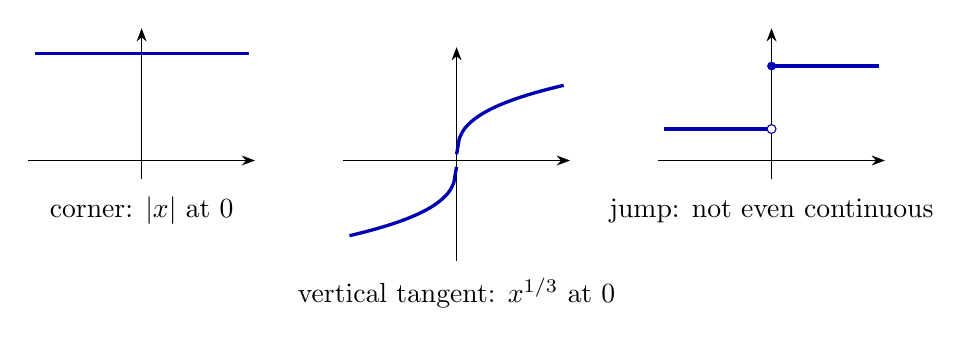
\begin{tikzpicture}[scale=0.8,>=Stealth]
\begin{scope}
\draw[->] (-1.8,0)--(1.8,0); \draw[->] (0,-0.3)--(0,2.1);
\draw[very thick,blue!70!black,domain=-1.7:1.7,samples=2] plot (\x,{abs(\x)});
\node at (0,-0.8) {corner: $|x|$ at $0$};
\end{scope}
\begin{scope}[xshift=5cm]
\draw[->] (-1.8,0)--(1.8,0); \draw[->] (0,-1.6)--(0,1.8);
\draw[very thick,blue!70!black,domain=0.001:1.7,samples=40] plot (\x,{\x^(1/3)});
\draw[very thick,blue!70!black,domain=0.001:1.7,samples=40] plot (-\x,{-(\x)^(1/3)});
\node at (0,-2.1) {vertical tangent: $x^{1/3}$ at $0$};
\end{scope}
\begin{scope}[xshift=10cm]
\draw[->] (-1.8,0)--(1.8,0); \draw[->] (0,-0.3)--(0,2.1);
\draw[very thick,blue!70!black] (-1.7,0.5)--(0,0.5); \draw[very thick,blue!70!black] (0,1.5)--(1.7,1.5);
\fill[white,draw=blue!70!black] (0,0.5) circle (2pt); \fill[blue!70!black] (0,1.5) circle (2pt);
\node at (0,-0.8) {jump: not even continuous};
\end{scope}
\end{tikzpicture}
\end{center}

\begin{example}[Standard cases]
\begin{itemize}[noitemsep]
\item $f(x)=|x|$ at $0$: right derivative $+1$, left derivative $-1$; not differentiable (corner), but continuous.
\item $f(x)=x^{1/3}$ at $0$: the difference quotient is $h^{-2/3}\to\infty$; vertical tangent, not differentiable.
\item $f(x)=x|x|$ at $0$: the quotient is $|h|\to0$, so $f'(0)=0$. Differentiable once (not twice).
\item $f(x)=x^2\sin\frac1x$ ($f(0)=0$): $\frac{f(h)}h=h\sin\frac1h\to0$, so $f'(0)=0$, yet $f'(x)=2x\sin\frac1x-\cos\frac1x$ has no limit at $0$. So $f'$ exists everywhere but is \emph{not continuous}.
\item $f(x)=x\sin\frac1x$ ($f(0)=0$): continuous at $0$ but $\frac{f(h)}h=\sin\frac1h$ oscillates, so not differentiable.
\end{itemize}
\end{example}

\subsection{Derivative rules}
\begin{formula}[Rules]
\begin{center}
\begin{tabular}{ll}
Sum, constant & $(af+bg)'=af'+bg'$\\
Product & $(fg)'=f'g+fg'$\\
Quotient & $\bigl(\frac fg\bigr)'=\frac{f'g-fg'}{g^2}$\\
Chain & $\bigl(f(g(x))\bigr)'=f'(g(x))\cdot g'(x)$\\
Inverse & $(f^{-1})'(y)=\frac1{f'(x)}$ where $y=f(x)$\\
Implicit & differentiate both sides w.r.t.\ $x$, treat $y$ as $y(x)$\\
Logarithmic & for $y=f^g$: $\ln y=g\ln f$, then differentiate
\end{tabular}
\end{center}
\end{formula}

\begin{formula}[Table of derivatives]
\begin{center}
\begin{tabular}{llll}
$(x^n)'=nx^{n-1}$ & $(e^x)'=e^x$ & $(a^x)'=a^x\ln a$ & $(\ln x)'=\frac1x$\\
$(\sin x)'=\cos x$ & $(\cos x)'=-\sin x$ & $(\tan x)'=\sec^2x$ & $(\sec x)'=\sec x\tan x$\\
$(\arcsin x)'=\frac1{\sqrt{1-x^2}}$ & $(\arccos x)'=-\frac1{\sqrt{1-x^2}}$ & $(\arctan x)'=\frac1{1+x^2}$ & $(\sinh x)'=\cosh x$
\end{tabular}
\end{center}
\end{formula}

\begin{example}[Derivatives that need care]
\begin{enumerate}[leftmargin=*,itemsep=4pt]
\item $y=x^x$ ($x>0$): $\ln y=x\ln x$, so $\frac{y'}y=\ln x+1$ and $y'=x^x(\ln x+1)$.
\item $y=x e^{-x}$: $y'=(1-x)e^{-x}$.
\item $y=\frac{\ln x}{x}$: $y'=\frac{1-\ln x}{x^2}$.
\item $y=\sigma(x)=\frac1{1+e^{-x}}$: $y'=\sigma(1-\sigma)$. Maximum slope $\frac14$ at $x=0$.
\item $y=\arctan x$: $y'=\frac1{1+x^2}$.
\item $y=x\ln x$: $y'=\ln x+1$.
\end{enumerate}
\end{example}

\subsection{Rolle's theorem and the Mean Value Theorem}
\begin{story}[The speed camera]
A speed camera at the start and another at the end of Ramu's trip recorded only his \emph{average} speed of $70$ km/h. Somu: ``At some moment on the way your speedometer read \emph{exactly} $70$.'' That is the \textbf{Mean Value Theorem}: the instantaneous rate must equal the average rate somewhere.
\end{story}
\begin{formula}[Theorems]
\begin{itemize}[noitemsep]
\item \textbf{Rolle:} if $f$ is continuous on $[a,b]$, differentiable on $(a,b)$ and $f(a)=f(b)$, then $f'(c)=0$ for some $c\in(a,b)$.
\item \textbf{MVT:} if $f$ is continuous on $[a,b]$ and differentiable on $(a,b)$, then there is $c\in(a,b)$ with $\displaystyle f'(c)=\frac{f(b)-f(a)}{b-a}$.
\item \textbf{Consequences:} $f'>0$ on an interval $\Rightarrow$ strictly increasing; $f'=0$ on an interval $\Rightarrow$ constant; $|f'|\le M\Rightarrow|f(x)-f(y)|\le M|x-y|$ (Lipschitz).
\end{itemize}
\end{formula}
\begin{example}[Finding $c$]
$f(x)=x^2$ on $[1,3]$: average slope $\frac{9-1}{2}=4$, and $f'(c)=2c=4$ gives $c=2$, which lies in $(1,3)$. For $f(x)=x^3-3x$ on $[-\sqrt3,\sqrt3]$: $f(\pm\sqrt3)=0$, and $f'(x)=3x^2-3=0$ gives $c=\pm1$ (Rolle).
\end{example}
\begin{trap}
(1) Differentiable $\Rightarrow$ continuous but not the converse; $|x|$ is the standard witness. (2) MVT fails for $|x|$ on $[-1,1]$: average slope $0$ but $f'$ is never $0$ (no derivative at $0$), because the hypothesis fails. (3) $f'(a)=0$ does \emph{not} imply a maximum or minimum ($x^3$ at $0$). (4) The chain rule applies from the outside in: $(\sin x^2)'=2x\cos x^2$, not $\cos x^2$.
\end{trap}
% =====================================================================
\section{Taylor Series}

\begin{story}[Zooming into a curvy road]
Ramu stands on a hilly road and asks Somu to describe it using only what he sees \emph{right here}. Somu: ``First I say: the road is at height $f(a)$. Better: it also slopes by $f'(a)$, so a straight line. Better still: it bends by $f''(a)$, so a parabola. Each extra derivative I know adds one more term and lets me predict the road a little farther away.'' That is a \textbf{Taylor polynomial}: it copies the function's height, slope, bend, and so on at one point.
\end{story}

\begin{formula}[Taylor and Maclaurin series]
If $f$ has derivatives of all orders at $a$,
\[f(x)=\sum_{k=0}^{\infty}\frac{f^{(k)}(a)}{k!}(x-a)^k=f(a)+f'(a)(x-a)+\frac{f''(a)}{2!}(x-a)^2+\frac{f'''(a)}{3!}(x-a)^3+\cdots\]
The special case $a=0$ is the \textbf{Maclaurin series}. The \textbf{Taylor polynomial of degree $n$} is the sum up to $k=n$; it is the \emph{unique} polynomial of degree $\le n$ that matches $f$ and its first $n$ derivatives at $a$.
\end{formula}

\begin{formula}[Lagrange remainder: how big is the error?]
$f(x)=P_n(x)+R_n(x)$ with
\[R_n(x)=\frac{f^{(n+1)}(c)}{(n+1)!}(x-a)^{n+1}\quad\text{for some }c\text{ between }a\text{ and }x.\]
So $|R_n|\le\dfrac{M}{(n+1)!}|x-a|^{n+1}$, where $M$ bounds $|f^{(n+1)}|$ between $a$ and $x$. The error shrinks quickly when $x$ is close to $a$ or $n$ is large. For $n=0$ this is exactly the Mean Value Theorem.
\end{formula}

\subsection{Standard Maclaurin series (memorise these)}
\begin{center}
\small
\renewcommand{\arraystretch}{1.7}
\begin{tabularx}{\textwidth}{>{\raggedright\arraybackslash}p{2.1cm}>{\raggedright\arraybackslash}X>{\raggedright\arraybackslash}p{2.2cm}}
\toprule
\textbf{Function} & \textbf{Series} & \textbf{Valid for}\\
\midrule
$e^x$ & $1+x+\frac{x^2}{2!}+\frac{x^3}{3!}+\frac{x^4}{4!}+\cdots=\sum\frac{x^k}{k!}$ & all $x$\\
$\sin x$ & $x-\frac{x^3}{3!}+\frac{x^5}{5!}-\frac{x^7}{7!}+\cdots$ & all $x$\\
$\cos x$ & $1-\frac{x^2}{2!}+\frac{x^4}{4!}-\frac{x^6}{6!}+\cdots$ & all $x$\\
$\frac1{1-x}$ & $1+x+x^2+x^3+\cdots$ & $|x|<1$\\
$\ln(1+x)$ & $x-\frac{x^2}{2}+\frac{x^3}{3}-\frac{x^4}{4}+\cdots$ & $-1<x\le1$\\
$\arctan x$ & $x-\frac{x^3}{3}+\frac{x^5}{5}-\frac{x^7}{7}+\cdots$ & $|x|\le1$\\
$(1+x)^\alpha$ & $1+\alpha x+\frac{\alpha(\alpha-1)}{2!}x^2+\frac{\alpha(\alpha-1)(\alpha-2)}{3!}x^3+\cdots$ & $|x|<1$\\
$\sqrt{1+x}$ & $1+\frac x2-\frac{x^2}{8}+\frac{x^3}{16}-\cdots$ & $|x|\le1$\\
$\tan x$ & $x+\frac{x^3}{3}+\frac{2x^5}{15}+\cdots$ & $|x|<\frac\pi2$\\
\bottomrule
\end{tabularx}
\end{center}

\begin{intuition}
\textbf{Patterns that save time.} \emph{Even} functions ($\cos x$) contain only even powers and \emph{odd} functions ($\sin x,\arctan x$) only odd powers. $\sin x$ and $\cos x$ alternate signs because their derivatives cycle $\sin\to\cos\to-\sin\to-\cos$. $\frac1{1-x}$ is the geometric series; replacing $x$ by $-x$ and integrating gives $\ln(1+x)$.
\end{intuition}

\begin{center}
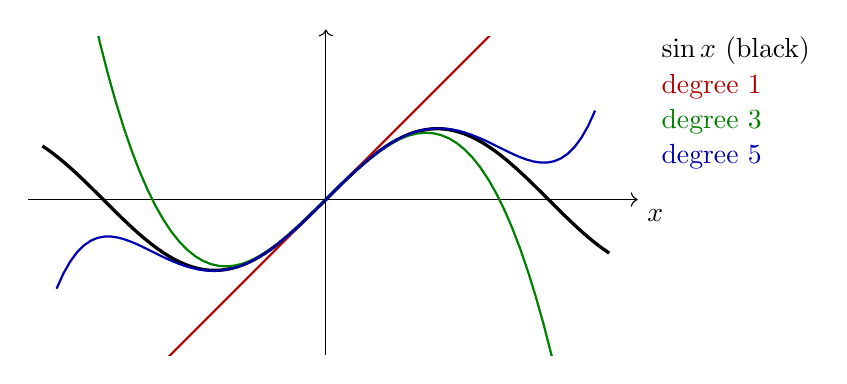
\begin{tikzpicture}[scale=0.9]
\draw[->] (-4.2,0)--(4.4,0) node[below right]{$x$}; \draw[->] (0,-2.2)--(0,2.4);
\begin{scope}
\clip (-4.2,-2.2) rectangle (4.2,2.3);
\draw[very thick,black,domain=-4:4,samples=100] plot (\x,{sin(\x r)});
\draw[thick,red!70!black,domain=-3:3,samples=60] plot (\x,{\x});
\draw[thick,green!50!black,domain=-3.3:3.3,samples=60] plot (\x,{\x-\x^3/6});
\draw[thick,blue!70!black,domain=-3.8:3.8,samples=80] plot (\x,{\x-\x^3/6+\x^5/120});
\end{scope}
\node[red!70!black,anchor=west] at (4.6,1.6) {degree 1};
\node[green!50!black,anchor=west] at (4.6,1.1) {degree 3};
\node[blue!70!black,anchor=west] at (4.6,0.6) {degree 5};
\node[anchor=west] at (4.6,2.1) {$\sin x$ (black)};
\end{tikzpicture}
\end{center}
Near $x=0$ all the polynomials hug $\sin x$; farther away the low-degree ones fly off while the degree-5 curve stays accurate longer.

\subsection{Worked examples}
\begin{example}[1. Taylor polynomial about a point other than 0]
$f(x)=x^3-2x+1$ about $a=1$: $f(1)=0$, $f'(x)=3x^2-2\Rightarrow f'(1)=1$, $f''(x)=6x\Rightarrow f''(1)=6$, $f'''=6$. So
\[f(x)=(x-1)+3(x-1)^2+(x-1)^3,\]
and the series stops: a polynomial is its own Taylor series.
\end{example}

\begin{example}[2. Approximations with error bounds]
\begin{itemize}[noitemsep]
\item $e^{0.5}$ with degree $3$: $1+0.5+0.125+0.0208333=1.6458333$ (true value $1.6487213$). Error bound: $\frac{e^{0.5}}{4!}(0.5)^4\le0.0043$; the actual error $0.0029$ is within the bound.
\item $\sqrt{1.1}$ with degree $2$ ($x=0.1$): $1+0.05-0.00125=1.04875$ (true $1.0488088$).
\item $\sin0.1$ with degree $3$: $0.1-\frac{0.001}{6}=0.0998333$ (true $0.0998334$).
\item $\ln1.2$ with degree $3$: $0.2-0.02+0.00267=0.18267$ (true $0.18232$).
\end{itemize}
\end{example}

\begin{example}[3. Limits by Taylor series: often faster than L'H\^opital]
\begin{itemize}[noitemsep]
\item $\displaystyle\lim_{x\to0}\frac{x-\sin x}{x^3}$: $x-\sin x=\frac{x^3}{6}-\cdots$, so the limit is $\frac16$.
\item $\displaystyle\lim_{x\to0}\frac{\cos x-1+\frac{x^2}2}{x^4}=\frac1{24}$ (the next term of $\cos x$).
\item $\displaystyle\lim_{x\to0}\frac{\tan x-x}{x^3}=\frac13$ (from $\tan x=x+\frac{x^3}3+\cdots$).
\item $\displaystyle\lim_{x\to0}\frac{e^x-1-x}{x^2}=\frac12$.
\end{itemize}
\end{example}

\begin{example}[4. Building new series from old ones]
\begin{itemize}[noitemsep]
\item \textbf{Substitute:} $e^{-x^2}=1-x^2+\frac{x^4}{2}-\cdots$ (replace $x$ by $-x^2$ in $e^x$).
\item \textbf{Multiply:} $e^x\sin x=(1+x+\frac{x^2}2+\cdots)(x-\frac{x^3}6+\cdots)=x+x^2+\frac{x^3}{3}+\cdots$
\item \textbf{Differentiate term by term:} $(\sin x)'=\cos x$ reproduces the cosine series.
\item \textbf{Integrate term by term:} integrating $\frac1{1+x^2}=1-x^2+x^4-\cdots$ gives $\arctan x$.
\item The coefficient of $x^k$ in a Maclaurin series equals $\frac{f^{(k)}(0)}{k!}$. So $f^{(5)}(0)$ for $\sin x$ is $5!\cdot\frac1{5!}=1$, and $f^{(4)}(0)$ for $e^{x}$ is $1$.
\end{itemize}
\end{example}

\subsection{Radius of convergence}
\begin{formula}[Ratio test]
For $\sum a_k(x-a)^k$ the \textbf{radius of convergence} is $R=\displaystyle\lim_{k\to\infty}\Bigl|\frac{a_k}{a_{k+1}}\Bigr|$. The series converges for $|x-a|<R$, diverges for $|x-a|>R$, and the endpoints must be checked separately. Examples: $\sum\frac{x^k}{k!}$: $R=\infty$; $\sum x^k$: $R=1$; $\sum\frac{x^k}{k}$ ($=-\ln(1-x)$): $R=1$, converges at $x=-1$, diverges at $x=1$.
\end{formula}

\begin{trap}
(1) Don't forget the factorial: the coefficient is $\frac{f^{(k)}(a)}{k!}$. (2) The series about $a$ uses powers of $(x-a)$, not $x$. (3) A function can have a Taylor series that converges but not to the function (e.g.\ $e^{-1/x^2}$ has all derivatives $0$ at $0$). (4) $\ln(1+x)$'s series needs $|x|\le1$, so you cannot use it directly for $\ln3$. (5) The $n$th-degree remainder involves the $(n+1)$st derivative.
\end{trap}

% =====================================================================
\section{Optimization of Single-variable Functions}

\begin{story}[Walking a hill in the fog]
Ramu and Somu climb a foggy hill. ``How do we know we are at a peak?'' Somu: ``At the top the ground is level for a moment: slope $=0$. Before the top you were walking uphill (slope $>0$), after it downhill (slope $<0$).'' Ramu: ``But a flat spot could also be a bench halfway up!'' ``Right, so we also look at how the slope itself changes: at a peak it keeps decreasing, so the second derivative is negative.''
\end{story}

\subsection{Terminology}
\begin{formula}[Definitions]
\begin{itemize}[noitemsep]
\item $x^*$ is a \textbf{local (relative) maximum} if $f(x^*)\ge f(x)$ for all $x$ near $x^*$; \textbf{global (absolute) maximum} if it holds for all $x$ in the domain. Minima are defined likewise.
\item A \textbf{critical point} is an interior point where $f'(x)=0$ or $f'(x)$ does not exist.
\item \textbf{Fermat's theorem:} if $f$ has a local extremum at an interior point where it is differentiable, then $f'(x^*)=0$. (So extrema hide among critical points and end points.)
\item $f$ is \textbf{concave up} (convex) where $f''>0$ and \textbf{concave down} where $f''<0$. An \textbf{inflection point} is where the concavity changes.
\end{itemize}
\end{formula}

\subsection{The tests}
\begin{formula}[First-derivative test]
At a critical point $c$: if $f'$ changes from $+$ to $-$, $c$ is a local maximum; from $-$ to $+$, a local minimum; no sign change, neither.
\end{formula}
\begin{formula}[Second-derivative test]
At a critical point with $f'(c)=0$: $f''(c)>0\Rightarrow$ local minimum; $f''(c)<0\Rightarrow$ local maximum; $f''(c)=0\Rightarrow$ \textbf{inconclusive} (use the first-derivative test or higher derivatives).\\
\textbf{Why:} near $c$, Taylor gives $f(c+h)\approx f(c)+\frac{f''(c)}2h^2$. If $f''(c)>0$ every nearby value is larger than $f(c)$: a valley.
\end{formula}
\begin{formula}[Higher-order test]
If $f'(c)=\dots=f^{(n-1)}(c)=0$ and $f^{(n)}(c)\ne0$: for \textbf{even} $n$ it is a local min ($f^{(n)}>0$) or max ($f^{(n)}<0$); for \textbf{odd} $n$ it is an inflection point (no extremum). Examples: $x^4$ at $0$ ($n=4$, minimum, although $f''(0)=0$); $x^3$ at $0$ ($n=3$, inflection).
\end{formula}

\begin{formula}[{Closed-interval method (global extrema of continuous $f$ on $[a,b]$)}]
Evaluate $f$ at (i) the end points $a,b$ and (ii) every critical point inside; the largest value is the global maximum and the smallest the global minimum. (The EVT guarantees they exist.)
\end{formula}

\begin{example}[Full analysis of $f(x)=x^3-6x^2+9x+1$]
$f'(x)=3x^2-12x+9=3(x-1)(x-3)$, so critical points $x=1,3$. $f''(x)=6x-12$.
\begin{center}
\begin{tabular}{c|ccc}
\toprule
interval & $x<1$ & $1<x<3$ & $x>3$\\
\midrule
sign of $f'$ & $+$ & $-$ & $+$\\
behaviour & increasing & decreasing & increasing\\
\bottomrule
\end{tabular}
\end{center}
$f''(1)=-6<0$: local \textbf{max} $f(1)=5$. $f''(3)=6>0$: local \textbf{min} $f(3)=1$. Inflection at $f''=0\Rightarrow x=2$.\\
On $[0,4]$: $f(0)=1,\ f(1)=5,\ f(3)=1,\ f(4)=5$. So the global max is $5$ (at $x=1$ and $x=4$) and the global min is $1$ (at $x=0$ and $x=3$).
\end{example}

\begin{center}
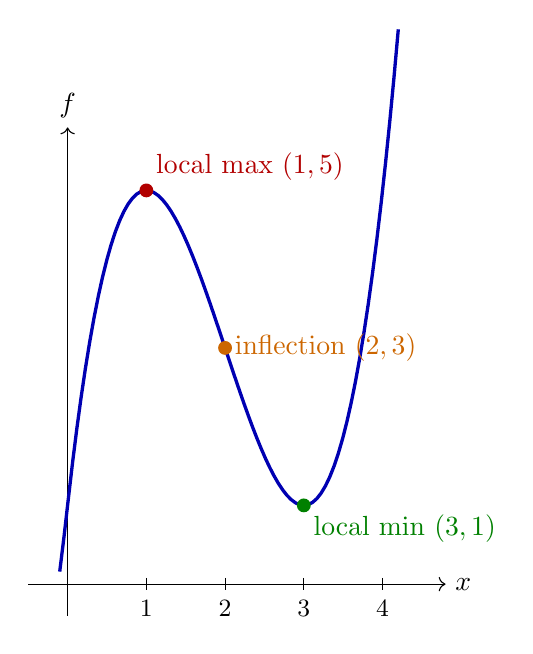
\begin{tikzpicture}[scale=1.0]
\draw[->] (-0.5,0)--(4.8,0) node[right]{$x$}; \draw[->] (0,-0.4)--(0,5.8) node[above]{$f$};
\draw[very thick,blue!70!black,domain=-0.1:4.2,samples=80] plot (\x,{\x^3-6*\x^2+9*\x+1});
\fill[red!70!black] (1,5) circle (2.5pt) node[above right]{local max $(1,5)$};
\fill[green!50!black] (3,1) circle (2.5pt) node[below right]{local min $(3,1)$};
\fill[orange!80!black] (2,3) circle (2.5pt) node[right]{inflection $(2,3)$};
\foreach \x in {1,2,3,4} \draw (\x,0.08)--(\x,-0.08) node[below]{\small\x};
\end{tikzpicture}
\end{center}

\begin{example}[Tricky critical points]
\begin{itemize}[noitemsep]
\item $f(x)=x e^{-x}$: $f'=(1-x)e^{-x}=0\Rightarrow x=1$; $f'$ goes $+\to-$: maximum $f(1)=\frac1e\approx0.368$.
\item $f(x)=x\ln x$ ($x>0$): $f'=\ln x+1=0\Rightarrow x=\frac1e$; $f''=\frac1x>0$: minimum $f(\frac1e)=-\frac1e$. (Used in the entropy function of information theory.)
\item $f(x)=\frac{\ln x}{x}$: $f'=\frac{1-\ln x}{x^2}=0\Rightarrow x=e$: maximum $\frac1e$. (So $e^{1/e}$ is the largest value of $x^{1/x}$.)
\item $f(x)=x+\frac1x$ for $x>0$: $f'=1-\frac1{x^2}=0\Rightarrow x=1$, minimum $2$ (AM--GM).
\item $f(x)=\sin x+\cos x$: maximum $\sqrt2$ at $x=\frac\pi4$.
\item $f(x)=x^3-3x$ on $[-2,3]$: values $f(-2)=-2$, $f(-1)=2$, $f(1)=-2$, $f(3)=18$. Global max $18$ at $x=3$; global min $-2$ at $x=-2$ and $x=1$.
\item $f(x)=|x|$: minimum at $0$ where $f'$ does not exist: a critical point of the second kind.
\item $f(x)=x^4-x^2+1$: $f'=4x^3-2x=2x(2x^2-1)=0\Rightarrow x=0,\pm\frac1{\sqrt2}$. Minima at $\pm\frac{1}{\sqrt2}$ with value $\frac34$; local maximum $1$ at $x=0$.
\end{itemize}
\end{example}

\subsection{Word problems: the recipe}
\begin{intuition}
(1) Draw and name the quantities. (2) Write the \textbf{objective} (what to maximise or minimise). (3) Write the \textbf{constraint} and use it to eliminate all but one variable. (4) State the domain. (5) Find critical points and compare with the end points. (6) Answer the question that was asked (units, the second quantity).
\end{intuition}

\begin{example}[Four classics]
\begin{enumerate}[leftmargin=*,itemsep=5pt]
\item \textbf{Rectangle with perimeter $40$.} $A=x(20-x)$, $A'=20-2x=0\Rightarrow x=10$; the maximum area is $100$ (a square).
\item \textbf{Farmer with 100 m of fence along a river} (no fence needed on the river side): $A=x(100-2x)$, $A'=100-4x=0\Rightarrow x=25$; width $25$, length $50$; area $1250$ m$^2$.
\item \textbf{Open box from a $12\times12$ sheet} by cutting squares of side $s$ from the corners: $V=s(12-2s)^2$, $V'=(12-2s)(12-6s)=0\Rightarrow s=2$ (since $s=6$ gives $V=0$). Maximum volume $V(2)=128$.
\item \textbf{Closed cylindrical can of volume $1000$ cm$^3$} with the least material: $A=2\pi r^2+\frac{2000}{r}$, $A'=4\pi r-\frac{2000}{r^2}=0\Rightarrow r^3=\frac{500}{\pi}$, $r\approx5.42$ cm, and then $h=\frac{1000}{\pi r^2}=2r$. The best can has height equal to its diameter.
\item \textbf{Closest point on $y=x^2$ to $(0,1)$.} Minimise $d^2=x^2+(x^2-1)^2=x^4-x^2+1$ (squaring avoids the root and has the same minimiser). Minimum at $x^2=\frac12$: $d^2=\frac34$, so $d=\frac{\sqrt3}2$.
\end{enumerate}
\end{example}

\subsection{Convexity: why optimisers love it}
\begin{formula}[Convex functions]
$f$ is \textbf{convex} on an interval if $f(\lambda x+(1-\lambda)y)\le\lambda f(x)+(1-\lambda)f(y)$ for all $0\le\lambda\le1$: every chord lies above the graph. For twice-differentiable $f$ this is equivalent to $f''\ge0$. For convex $f$:
\begin{itemize}[noitemsep]
\item every critical point is a \textbf{global minimum} (no local-versus-global worry); $f(y)\ge f(x)+f'(x)(y-x)$: the tangent line lies below the graph;
\item Jensen's inequality: $f(\mathbb E[X])\le\mathbb E[f(X)]$.
\end{itemize}
Examples of convex functions: $x^2$, $e^x$, $|x|$, $-\ln x$, $x\ln x$. Squared-error loss and logistic loss in machine learning are convex, which is why training them is reliable.
\end{formula}

\subsection{Numerical methods that come from calculus}
\begin{story}[Rolling a ball downhill]
Ramu is told to find the lowest point of $f(x)=(x-3)^2$ without algebra. Somu: ``Stand anywhere, look at the slope, and step \emph{against} it: $x_{k+1}=x_k-\eta f'(x_k)$. The number $\eta>0$ is the \textbf{learning rate}.'' This is \textbf{gradient descent}.
\end{story}
For $f=(x-3)^2$ we have $f'=2(x-3)$, so $x_{k+1}-3=(1-2\eta)(x_k-3)$. Starting from $x_0=0$ with $\eta=0.1$ (factor $0.8$):
\begin{center}
\begin{tabular}{c|cccccc}
\toprule
$k$ & 0 & 1 & 2 & 3 & 4 & 5\\
\midrule
$x_k$ & 0 & 0.6 & 1.08 & 1.464 & 1.7712 & 2.017\\
\bottomrule
\end{tabular}
\end{center}
The iterates creep toward $3$. The method converges iff $|1-2\eta|<1$, i.e.\ $0<\eta<1$; for $\eta=1$ it bounces between $0$ and $6$ forever, and for $\eta>1$ it diverges. In general the step size must be below $\frac2L$ where $L$ bounds $f''$.

\begin{formula}[Newton's method]
\textbf{Root finding:} $x_{k+1}=x_k-\dfrac{f(x_k)}{f'(x_k)}$ (follow the tangent line to the axis). Example $f=x^2-2$, $x_0=1$: $x_1=1.5$, $x_2=1.41667$, $x_3=1.41422$, $x_4=1.41421\to\sqrt2$. The number of correct digits roughly \emph{doubles} each step (quadratic convergence).\\
\textbf{Optimisation:} apply it to $f'$: $x_{k+1}=x_k-\dfrac{f'(x_k)}{f''(x_k)}$; it uses the curvature to choose the step. For a quadratic it lands on the minimum in one step.
\end{formula}

\begin{trap}
(1) $f'(c)=0$ does not guarantee an extremum ($x^3$). (2) $f''(c)=0$ does not rule one out ($x^4$). (3) Global extrema on a closed interval may be at the end points, where $f'\ne0$. (4) On an open interval a maximum may not exist at all. (5) Check the domain: $x\ln x$ needs $x>0$. (6) In word problems verify that the critical point is really a max or min and not a boundary or a zero-volume case. (7) A local min of a non-convex function need not be a global min.
\end{trap}

% =====================================================================
\newpage
\part{Previous-Year Questions: GATE DA 2024, 2025, 2026}

\section{How to Use the Past Papers}

\begin{story}[Ramu asks: what do they really ask from calculus?]
Ramu: ``Somu, calculus has limits, Taylor series, optimisation and so much more. Which parts show up?'' Somu opens the three GATE DA papers and lists every question from this section. He solves each, names the idea behind it, and points to the chapter that teaches it. The surprise: the questions are short, and almost all of them have a one-line trick.
\end{story}

\begin{formula}[Facts from the official papers and answer keys (verified)]
\begin{center}
\begin{tabular}{lccc}
\toprule
 & \textbf{2024} & \textbf{2025} & \textbf{2026}\\\midrule
Calculus \& Optimization questions & 5 & 7 & 3\\
1-mark / 2-mark & 2\,/\,3 & 3\,/\,4 & 3\,/\,0\\
Marks from this section & 8 & 11 & 3\\
\bottomrule
\end{tabular}
\end{center}
\textbf{15 questions} in all. Question numbers: 2024: 15, 33, 37, 50, 60. 2025: 14, 24, 32, 48, 49, 51, 59. 2026: 27, 29, 35. Types: MCQ, MSQ (select all that apply) and NAT (type a number).\\
\textbf{Source note.} The 2024 and 2026 questions are restated from the official IIT papers; every answer is the official key's. The official 2025 paper file could not be opened here, so the 2025 wording is restated from a published solution set; its answers agree with the official 2025 key and with my own computations. In the 2025 Q49 statement the constant $2133$ was reconstructed from that source (the answers do not depend on it).
\end{formula}

\subsection{Where the 15 questions come from}
\begin{center}
\small
\begin{tabularx}{\textwidth}{>{\raggedright\arraybackslash}p{5.0cm}cX}
\toprule
\textbf{Topic group} & \textbf{Count} & \textbf{Questions (year-Q)}\\\midrule
A. Limits & 2 & 24-Q60; 25-Q32\\
B. Continuity and differentiability & 4 & 24-Q37; 25-Q24, Q48, Q59\\
C. Derivatives, Taylor and series & 3 & 24-Q33; 25-Q14; 26-Q35\\
D. Optimisation (extrema, convexity, gradient descent) & 6 & 24-Q15, Q50; 25-Q49, Q51; 26-Q27, Q29\\
\bottomrule
\end{tabularx}
\end{center}
\textbf{Reading the pattern.} Optimisation is the biggest group (6 of 15), and two of them (26-Q29 and 24-Q33) are secretly \emph{machine learning} questions: a gradient-descent step and the derivative of the sigmoid. ReLU (25-Q48) and sigmoid (24-Q33) appear because they are the building blocks of neural networks. Expect GATE DA to keep dressing ML objects in calculus clothes.

\subsection{The concept map}
\begin{center}
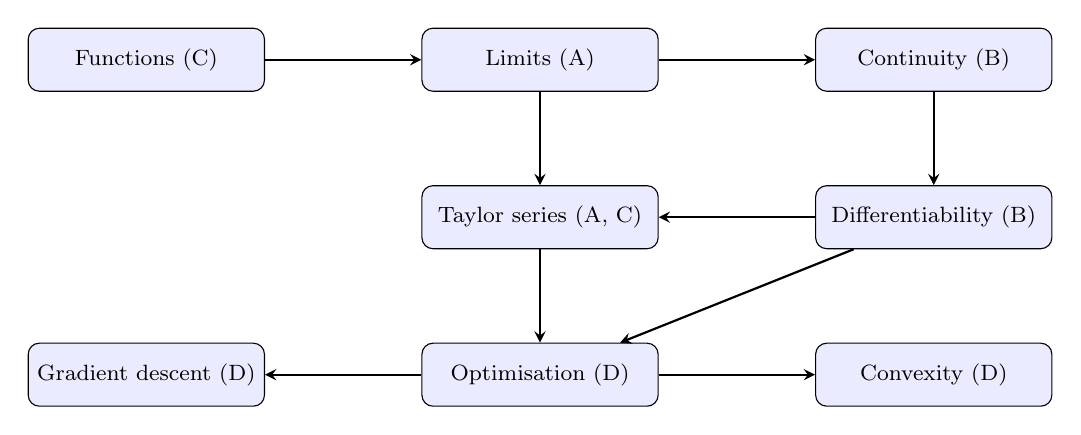
\begin{tikzpicture}[
 b/.style={draw,rounded corners,fill=blue!8,minimum height=8mm,minimum width=30mm,align=center,font=\footnotesize,inner sep=3pt},
 a/.style={->,thick,>=stealth}]
\node[b] (fn) at (0,0) {Functions (C)};
\node[b] (lim) at (5,0) {Limits (A)};
\node[b] (con) at (10,0) {Continuity (B)};
\node[b] (dif) at (10,-2) {Differentiability (B)};
\node[b] (tay) at (5,-2) {Taylor series (A, C)};
\node[b] (opt) at (5,-4) {Optimisation (D)};
\node[b] (cvx) at (10,-4) {Convexity (D)};
\node[b] (gd) at (0,-4) {Gradient descent (D)};
\draw[a](fn)--(lim);\draw[a](lim)--(con);\draw[a](con)--(dif);\draw[a](dif)--(tay);
\draw[a](lim)--(tay);\draw[a](dif)--(opt);\draw[a](tay)--(opt);\draw[a](opt)--(cvx);\draw[a](opt)--(gd);
\end{tikzpicture}
\end{center}

% =====================================================================
\section{Group A: Limits (2 questions)}

\begin{story}[Two weapons: conjugates and Taylor series]
Somu: ``Almost every GATE limit falls to one of two tools. If the expression has a square root, \emph{multiply by the conjugate}. If it has $\ln$, $\cos$, $e^x$ near $0$, \emph{replace each by its first Taylor terms}.''
\end{story}

\begin{example}[2024 Q60 (2 marks, NAT): $\displaystyle\lim_{x\to0}\frac{\ln\bigl((x^2+1)\cos x\bigr)}{x^2}$]
Split the logarithm: $\ln(1+x^2)+\ln\cos x$. Near $0$: $\ln(1+x^2)=x^2-\frac{x^4}2+\dots$ and $\cos x=1-\frac{x^2}2+\dots$, so $\ln\cos x=-\frac{x^2}2+O(x^4)$. Sum $=x^2-\frac{x^2}2+O(x^4)=\frac{x^2}2+\dots$ (the computer algebra series is $\frac{x^2}2-\frac{7x^4}{12}+\dots$). Dividing by $x^2$:
\[\lim=1-\frac12=\mathbf{\tfrac12}\quad(\text{key: }0.5).\]
\textbf{L'H\^opital alternative:} the form is $\frac00$; differentiate top and bottom: $\frac{\frac{2x}{x^2+1}-\tan x}{2x}\to\frac{2x-x}{2x}=\frac12$. Same answer, but Taylor is faster.\\
\textbf{Connect:} Taylor chapter, standard series for $\ln(1+u)$ and $\cos x$; the limit equals the coefficient of $x^2$ in the numerator.
\end{example}

\begin{example}[2025 Q32 (1 mark, NAT): $\displaystyle\lim_{t\to\infty}\bigl(\sqrt{t^2+t}-\sqrt{t^2+1}\bigr)$]
Form $\infty-\infty$. Multiply and divide by the conjugate:
\[\frac{(t^2+t)-(t^2+1)}{\sqrt{t^2+t}+\sqrt{t^2+1}}=\frac{t-1}{\sqrt{t^2+t}+\sqrt{t^2+1}}.\]
Divide by $t$: $\dfrac{1-1/t}{\sqrt{1+1/t}+\sqrt{1+1/t^2}}\to\dfrac{1}{1+1}=\mathbf{0.5}$.\\
\textbf{Rule:} an $\infty-\infty$ with square roots is almost always the conjugate trick; then divide by the highest power.
\end{example}

\begin{trap}
(1) Do not substitute $x=0$ into a $\frac00$ form and stop. (2) When using Taylor, keep enough terms: the first term that does \emph{not} cancel decides the limit. (3) L'H\^opital only applies to $\frac00$ or $\frac\infty\infty$, and the derivative limit must exist.
\end{trap}

% =====================================================================
\section{Group B: Continuity and Differentiability (4 questions)}

\begin{story}[Smooth gluing]
Ramu: ``Two curves are joined at a point. How do I make the joint \emph{smooth}?'' Somu: ``Two conditions at every joint: the \emph{values} agree (continuity), and the \emph{slopes} agree (differentiability). Write both as equations and solve.''
\end{story}

\begin{formula}[Rules used in Group B]
Differentiable $\Rightarrow$ continuous (not conversely: $|x|$). Sum, difference, product of differentiable functions are differentiable; quotient too if the denominator is non-zero; a composition $f\circ g$ is differentiable at $c$ if $g$ is differentiable at $c$ \emph{and $f$ is differentiable at $g(c)$}. A piecewise function is differentiable at a joint $c$ iff the left and right values \emph{and} the left and right derivatives agree.
\end{formula}

\begin{example}[2024 Q37 (2 marks, MCQ): gluing a parabola to two lines]
$f=-x$ for $x<-2$; $ax^2+bx+c$ on $[-2,2]$; $f=x$ for $x>2$. At $x=2$: continuity $4a+2b+c=2$, slope $4a+b=1$. At $x=-2$: value of the left piece is $-(-2)=2$, so $4a-2b+c=2$; slope of the left piece is $-1$, so $-4a+b=-1$. Adding the slope equations: $2b=0\Rightarrow b=0$, then $a=\frac14$, and $c=2-4a=1$. Answer \textbf{(A)} $a=\frac14,b=0,c=1$. Checking the other options: (B) $(\frac12,0,0)$ gives slope $4a+b=2\ne1$; (C) fails continuity; (D) fails continuity at $x=-2$ ($4-2-4=-2\ne2$).\\
\textbf{Method:} four equations, three unknowns; the symmetry makes one redundant. The resulting function is $f(x)=\frac{x^2}4+1$ on $[-2,2]$, which is tangent to both lines (it is the smooth ``rounded absolute value'').
\end{example}

\begin{example}[2025 Q24 (1 mark, MSQ): combining differentiable functions]
$f:\R\to\R$ and $g:\R\to(1,\infty)$ are differentiable at $c$.
\begin{itemize}[noitemsep]
\item (A) $f\pm g$: \textbf{yes}. (B) $f\cdot g$: \textbf{yes}.
\item (C) $f/g$: \textbf{yes}, because $g>1$ so it is never $0$.
\item (D) $f\circ g+g\circ f$: \emph{not guaranteed}. The chain rule needs $f$ differentiable \emph{at the point $g(c)$}, but we only know $f$ is differentiable at $c$. Likewise $g\circ f$ needs $g$ differentiable at $f(c)$, but $g$ is only known to be differentiable at $c$.
\end{itemize}
Answer: A, B, C. \textbf{Trap:} the range $(1,\infty)$ is there to make the denominator safe.
\end{example}

\begin{example}[2025 Q48 (2 marks, MSQ): ReLU]
$\mathrm{ReLU}(x)=\max(x,0)$. (a) Continuous everywhere: \textbf{true} (both pieces meet at $0$ with value $0$). (b) Differentiable everywhere: \emph{false}. (c) Not differentiable at $0$: \textbf{true}. The left derivative is $0$ and the right derivative is $1$, which differ. (d) $\mathrm{ReLU}(x)=\mathrm{ReLU}(ax)$ for all real $a$: \emph{false}; with $a=-1$, $x=1$: $\mathrm{ReLU}(1)=1$ but $\mathrm{ReLU}(-1)=0$. Answer: A, C.\\
\textbf{Connect:} neural networks use ReLU even though it has a kink; in practice one picks a sub-gradient ($0$ or $1$) at $x=0$.
\end{example}

\begin{example}[2025 Q59 (2 marks, NAT): a function squeezed between $0$ and $(x-y)^2$]
$|f(x)-f(y)|\le(x-y)^2$ for all $x,y$. Divide by $|x-y|$:
\[\left|\frac{f(x)-f(y)}{x-y}\right|\le|x-y|\xrightarrow[y\to x]{}0\ \Rightarrow\ f'(x)=0\ \text{for every }x.\]
A function with zero derivative everywhere is constant (by the Mean Value Theorem), so $f(1)-f(0)=\mathbf0$.\\
\textbf{Lesson:} a ``H\"older bound'' with exponent greater than $1$ forces a constant function. With $|x-y|$ (exponent $1$) the function could be $f(x)=x$.
\end{example}

\begin{trap}
(1) Check \emph{both} value and slope at every joint. (2) The chain rule requires differentiability at the \emph{inner function's value}. (3) $|x|$ and $\mathrm{ReLU}$ are continuous but not differentiable at $0$. (4) Differentiability implies continuity, never the reverse.
\end{trap}

% =====================================================================
\section{Group C: Derivatives, Taylor Coefficients, Series (3 questions)}

\begin{example}[2024 Q33 (1 mark, NAT): derivative of the sigmoid]
$f(x)=\dfrac1{1+e^{-x}}$. Its derivative is $f'(x)=f(x)\bigl(1-f(x)\bigr)$ (prove: $f'=\frac{e^{-x}}{(1+e^{-x})^2}=f\cdot\frac{e^{-x}}{1+e^{-x}}=f(1-f)$). The question asks for $f'$ where $f=0.4$, so we do not need $x$ at all:
\[f'=0.4\times0.6=\mathbf{0.24}\quad(\text{key: }0.24).\]
(The corresponding $x$ is $\ln\frac{0.4}{0.6}=-0.405$.) \textbf{Connect:} the maximum of $f(1-f)$ is $0.25$ at $f=\frac12$; this is why sigmoid gradients are small for large $|x|$ (the ``vanishing gradient'' of deep learning).
\end{example}

\begin{example}[2025 Q14 (1 mark, MCQ): the $10$th derivative of $\sinh x$ at $0$]
$f(x)=\dfrac{e^x-e^{-x}}2=\sinh x$. Its Maclaurin series has only \emph{odd} powers: $x+\frac{x^3}{3!}+\frac{x^5}{5!}+\cdots$. The coefficient of $x^{10}$ is $0$, and $f^{(10)}(0)=10!\cdot0=\mathbf0$ \quad (A). Check by differentiating: derivatives alternate $\cosh x,\sinh x,\cosh x,\dots$ and the even-order ones are $\sinh$, which vanish at $0$.\\
\textbf{Method:} $f^{(n)}(0)=n!\times(\text{coefficient of }x^n)$. Odd function $\Rightarrow$ even-order derivatives at $0$ are $0$.
\end{example}

\begin{example}[2026 Q35 (1 mark, NAT): a double geometric series]
$\displaystyle\sum_{i=0}^\infty\sum_{j=1}^\infty2^{-i}3^{-j}$. The terms factor, so the double sum is a product of two geometric sums:
\[\sum_{i\ge0}2^{-i}=\frac1{1-\frac12}=2,\qquad\sum_{j\ge1}3^{-j}=\frac{\frac13}{1-\frac13}=\frac12,\qquad\text{product}=\mathbf1.\]
Note the starting indices: $i$ starts at $0$ (first term $1$), $j$ starts at $1$ (first term $\frac13$). \textbf{Formula:} $\sum_{k\ge m}r^k=\dfrac{r^m}{1-r}$ for $|r|<1$.
\end{example}

% =====================================================================
\section{Group D: Optimisation (6 questions)}

\begin{story}[Where the hill flattens]
Ramu: ``How do I find the top of a hill?'' Somu: ``Walk until the ground is flat ($f'=0$). Then check the curvature: bending down ($f''<0$) is a peak, bending up ($f''>0$) is a valley. On a closed interval also check the two ends.''
\end{story}

\begin{formula}[Tests]
\textbf{Second-derivative test} at a stationary point $c$ ($f'(c)=0$): $f''(c)>0\Rightarrow$ local minimum; $f''(c)<0\Rightarrow$ local maximum; $f''(c)=0\Rightarrow$ test fails (examples $x^3$ and $x^4$). \textbf{Closed interval $[a,b]$:} compare $f$ at the endpoints and at all stationary points. \textbf{Convex} ($f''\ge0$): every stationary point is a global minimum. \textbf{Gradient descent:} $w\leftarrow w-\eta f'(w)$.
\end{formula}

\begin{example}[2024 Q15 (1 mark, MCQ): $f'(x^*)=0$ and $f''(x^*)>0$]
This is exactly the second-derivative test: a \textbf{local minimum} \quad (A). It need not be global: $f(x)=x^4-x^2+\frac x{10}$ has two local minima, only one of them global. Likewise $f'=0,f''<0$ is a local maximum.
\end{example}

\begin{example}[2024 Q50 (2 marks, MSQ): quartic $f=\frac{x^4}4-\frac{2x^3}3-\frac{3x^2}2+1$]
$f'(x)=x^3-2x^2-3x=x(x-3)(x+1)$, stationary points $x=-1,0,3$. $f''(x)=3x^2-4x-3$:
\[f''(-1)=4>0\ (\text{local min}),\qquad f''(0)=-3<0\ (\text{local max}),\qquad f''(3)=12>0\ (\text{local min}).\]
(A) $x=0$ local maximum: \textbf{true}. (B) $x=3$ local minimum: \textbf{true}. (C) $x=-1$ local maximum: \emph{false}, it is a minimum. (D) $x=0$ local minimum: \emph{false}. Answer: A, B.
\end{example}

\begin{example}[2025 Q49 (2 marks, MSQ): extrema of a cubic on a closed interval]
$f(x)=\frac{x^3}3+\frac{7x^2}2+10x+2133$ on $[-8,0]$. $f'(x)=x^2+7x+10=(x+2)(x+5)$, so stationary points $x=-5$ (local max) and $x=-2$ (local min). Compare values: $f(-8)=2106.33$, $f(-5)=2128.83$, $f(-2)=2124.33$, $f(0)=2133$. So on $[-8,0]$ the \textbf{global maximum is $2133$ at the endpoint $x=0$} and the global minimum is at the endpoint $x=-8$.
\begin{itemize}[noitemsep]
\item (a) maximum at $x=-5$: \emph{false} (local only). (b) minimum at $x=-2$: \emph{false} (local only).
\item (c) maximum value is $2133$: \textbf{true}.
\item (d) the minimum of $f'$ occurs at $x=-\frac72$: $f''(x)=2x+7=0$ at $x=-\frac72$, inside the interval, and $f'(-\frac72)=-\frac94$ is the least value of $f'$. \textbf{True.}
\end{itemize}
Answer: C, D. \textbf{Lesson:} on a closed interval, the maximum can sit at an endpoint, which a pure derivative test never sees.
\end{example}

\begin{example}[2025 Q51 (2 marks, MSQ): $f''>0$ everywhere]
$f''>0\Rightarrow f'$ is strictly increasing, so $f'$ can be $0$ at \emph{most once}. Hence (b) ``no two distinct points have $f'=0$'' \textbf{true}; (c) ``at most one global minimum'' \textbf{true}; (d) ``at most one local minimum'' \textbf{true}. (a) ``$f$ has a local minimum'': \emph{false}, $f(x)=e^x$ has $f''>0$ but never a stationary point. Answer: B, C, D.\\
\textbf{Connect:} strictly convex functions have at most one minimiser, which is why least-squares and logistic regression have unique solutions.
\end{example}

\begin{example}[2026 Q27 (1 mark, MSQ): a cubic on a half-open interval]
$f(x)=x^3-3x^2+2$ on $(-1,3]$. Roots: $x=1$ is a root ($1-3+2=0$); factoring gives $(x-1)(x^2-2x-2)$ with the other roots $1\pm\sqrt3=-0.732$ and $2.732$. $f'(x)=3x^2-6x=3x(x-2)$: stationary points $0$ (local max, value $2$) and $2$ (local min, value $-2$). Endpoint values: $f(3)=2$; $x=-1$ is \emph{excluded} (and $f(-1)=-2$).
\begin{itemize}[noitemsep]
\item (A) exactly two roots in $[-0.9,0]$: \emph{false}, only $-0.732$.
\item (B) minimum only at $x=2$: \textbf{true}. The global minimum value is $-2$; it would also be attained at $x=-1$, but that point is not in the domain.
\item (C) maximum only at $x=0$: \emph{false}, $f(3)=2=f(0)$ as well.
\item (D) root at $x=1$: \textbf{true}.
\end{itemize}
Answer: B, D. \textbf{Trap:} read whether each end of the interval is open or closed.
\end{example}

\begin{example}[2026 Q29 (1 mark, NAT): one step of stochastic gradient descent]
The objective is $f_w(x)=wx$, so $\dfrac{\partial f}{\partial w}=x$. One SGD step: $w\leftarrow w-\eta\,\dfrac{\partial f}{\partial w}=10-0.10\times10=\mathbf{9.00}$ (key: $8.90$ to $9.10$). Nothing else is needed: the loss is the function $wx$ itself, no label is involved.\\
\textbf{Connect:} gradient descent is the numerical optimisation method of this chapter; the next chapter (Machine Learning) uses the same update on real losses.
\end{example}

\begin{trap}
(1) The second-derivative test says nothing when $f''=0$. (2) A local minimum is not automatically global. (3) On closed intervals check the endpoints; on open or half-open ones the missing endpoint cannot be an extremum. (4) Strict convexity gives \emph{at most one} stationary point, not necessarily one.
\end{trap}

% =====================================================================
\section{Six Ideas that Solved the 15 Questions}
\begin{formula}[Connecting the dots]
\begin{enumerate}[noitemsep]
\item \textbf{Conjugate or Taylor} for limits (24-Q60, 25-Q32).
\item \textbf{Glue conditions:} equal value and equal slope at each joint (24-Q37); kink functions such as ReLU are continuous but not differentiable (25-Q48).
\item \textbf{Differentiability closure rules} and the chain-rule condition (25-Q24); a bound $(x-y)^2$ forces $f'=0$ (25-Q59).
\item \textbf{Taylor coefficients} give derivatives: $f^{(n)}(0)=n!\,a_n$ (25-Q14); geometric series $\sum r^k$ (26-Q35); $\sigma'=\sigma(1-\sigma)$ (24-Q33).
\item \textbf{Stationary points and the second-derivative test}, then compare endpoints (24-Q15, Q50; 25-Q49; 26-Q27).
\item \textbf{Convexity:} $f''>0$ means at most one minimiser (25-Q51); \textbf{gradient descent} $w\leftarrow w-\eta f'$ (26-Q29).
\end{enumerate}
\end{formula}

\begin{center}
\small
\begin{tabularx}{\textwidth}{>{\raggedright\arraybackslash}p{2.7cm}>{\raggedright\arraybackslash}X>{\raggedright\arraybackslash}p{3.4cm}}
\toprule
\textbf{Question (answer)} & \textbf{Idea in one line} & \textbf{Notes chapter}\\\midrule
24-Q15 (A) & $f'=0,f''>0$: local min & Optimisation\\
24-Q33 ($0.24$) & $\sigma'=\sigma(1-\sigma)$ & Derivatives\\
24-Q37 (A) & value and slope match at joints & Differentiability\\
24-Q50 (A,B) & second-derivative test & Optimisation\\
24-Q60 ($0.5$) & Taylor of $\ln(1+x^2)+\ln\cos x$ & Limits, Taylor\\
25-Q14 (A, $0$) & even-order derivative of odd function & Taylor series\\
25-Q24 (A,B,C) & closure of differentiable functions & Differentiability\\
25-Q32 ($0.5$) & conjugate trick & Limits\\
25-Q48 (A,C) & ReLU kink & Continuity, differentiability\\
25-Q49 (C,D) & closed interval, endpoint maximum & Optimisation\\
25-Q51 (B,C,D) & $f''>0\Rightarrow f'$ strictly increasing & Convexity\\
25-Q59 ($0$) & $|f(x)-f(y)|\le(x-y)^2\Rightarrow f'=0$ & MVT, differentiability\\
26-Q27 (B,D) & roots, extrema, open interval & Optimisation\\
26-Q29 ($9.00$) & $w-\eta\,\partial f/\partial w$ & Numerical methods\\
26-Q35 ($1$) & product of geometric sums & Series\\
\bottomrule
\end{tabularx}
\end{center}

% =====================================================================
\newpage
\part{Deeper Explanations: Proofs and Intuition}

\section{Why the Key Facts are True}

\begin{story}[Ramu insists on ``why'']
Ramu: ``I can apply the second-derivative test and the Taylor series, but why do they work?'' Somu: ``Each one is a small picture. Let us draw them.''
\end{story}

\subsection{Limits: what they mean and the standard ones}
\begin{formula}[Meaning, laws and the standard limits]
$\lim_{x\to a}f(x)=L$ means: for every $\varepsilon>0$ there is $\delta>0$ such that $0<|x-a|<\delta\Rightarrow|f(x)-L|<\varepsilon$. Limits respect sums, products and quotients (denominator limit $\neq0$). \textbf{Squeeze theorem:} $g\le f\le h$ and $g,h\to L\Rightarrow f\to L$.\\
\textbf{Why $\frac{\sin x}{x}\to1$:} for small $x>0$, comparing areas gives $\sin x<x<\tan x$; divide by $\sin x$: $\cos x<\frac{\sin x}x<1$, and the squeeze gives $1$. From it: $\frac{1-\cos x}{x^2}=\frac{\sin^2x}{x^2(1+\cos x)}\to\frac12$.\\
\textbf{Taylor makes limits easy} (verified): $\dfrac{e^x-1-x}{x^2}\to\dfrac12$, $\quad\dfrac{x-\sin x}{x^3}\to\dfrac16$, $\quad\dfrac{1-\cos x}{x^2}\to\dfrac12$. The limit is the ratio of the first non-cancelling coefficients.\\
\textbf{Other standard results:} $\lim_{x\to\infty}(1+\frac1x)^x=e$, $\ (1+\frac2x)^x\to e^2$, $\ \frac{\sin3x}x\to3$, $\ \frac{e^{2x}-1}{x}\to2$, $\ x\ln x\to0$ as $x\to0^+$, $\ \frac{\ln x}{x}\to0$ as $x\to\infty$.
\end{formula}
\begin{example}[Choosing the tool]
\begin{itemize}[noitemsep]
\item Square roots with $\infty-\infty$: conjugate (2025 Q32).
\item $\frac00$ with $\ln,\cos,e^x$ near $0$: Taylor (2024 Q60).
\item Polynomial ratios at $\infty$: divide by the highest power.
\item $0\cdot\infty$ or $\infty^0$: rewrite as a quotient, or take $\ln$.
\end{itemize}
\end{example}

\subsection{Continuity versus differentiability}
\begin{formula}[Relationships with proofs]
\textbf{Differentiable $\Rightarrow$ continuous:} $f(x)-f(a)=\frac{f(x)-f(a)}{x-a}(x-a)\to f'(a)\cdot0=0$. \textbf{Converse false:} $|x|$ and ReLU at $0$ have different left and right slopes. \textbf{A subtler example:} $f(x)=x^2\sin\frac1x$ ($f(0)=0$) is differentiable at $0$ with $f'(0)=\lim x\sin\frac1x=0$ (verified), but $f'$ is not continuous at $0$. So differentiable does not mean continuously differentiable.\\
\textbf{Smooth gluing:} to join pieces $f_1$ (left) and $f_2$ (right) at $c$, impose $f_1(c)=f_2(c)$ ($C^0$) and $f_1'(c)=f_2'(c)$ ($C^1$); for a $C^2$ join also $f_1''(c)=f_2''(c)$.\\
\textbf{Closure:} if $f,g$ are differentiable at $c$ then so are $f\pm g$, $fg$, $f/g$ (if $g(c)\ne0$). For compositions, $(f\circ g)'(c)=f'(g(c))\,g'(c)$ needs $f$ differentiable at $g(c)$.
\end{formula}
\begin{formula}[Rolle, the Mean Value Theorem and why they matter]
\textbf{MVT:} $f$ continuous on $[a,b]$ and differentiable on $(a,b)$ $\Rightarrow$ there is $c\in(a,b)$ with $f'(c)=\dfrac{f(b)-f(a)}{b-a}$ (the tangent is parallel to the chord). \textbf{Consequences:} $f'\equiv0\Rightarrow f$ constant (2025 Q59); $f'>0\Rightarrow f$ strictly increasing; $|f'|\le K\Rightarrow|f(x)-f(y)|\le K|x-y|$ (Lipschitz). \textbf{Intermediate Value Theorem:} a continuous $f$ on $[a,b]$ takes every value between $f(a)$ and $f(b)$ (used to prove roots exist); \textbf{Extreme Value Theorem:} a continuous function on a closed bounded interval attains a maximum and a minimum.
\end{formula}

\subsection{Taylor series and the size of the error}
\begin{formula}[Taylor's theorem with Lagrange remainder]
\[f(x)=\sum_{k=0}^n\frac{f^{(k)}(a)}{k!}(x-a)^k+R_n,\qquad R_n=\frac{f^{(n+1)}(\xi)}{(n+1)!}(x-a)^{n+1}\ \ (\xi\text{ between }a\text{ and }x).\]
Matching coefficients gives $f^{(k)}(a)=k!\,a_k$. Standard series (Maclaurin, $a=0$): $e^x=\sum\frac{x^k}{k!}$, $\sin x=x-\frac{x^3}{3!}+\dots$, $\cos x=1-\frac{x^2}{2!}+\dots$, $\ln(1+x)=x-\frac{x^2}2+\frac{x^3}3-\dots$ ($-1<x\le1$), $\frac1{1-x}=\sum x^k$ ($|x|<1$), $\sinh x=x+\frac{x^3}{3!}+\dots$. \textbf{Even function} $\Rightarrow$ only even powers; \textbf{odd function} $\Rightarrow$ only odd powers (so odd-order derivatives of an even function vanish at $0$, and the reverse).
\end{formula}
\begin{example}[How good is a short Taylor polynomial? (computed)]
$\sin0.5\approx0.5-\frac{0.5^3}6+\frac{0.5^5}{120}=0.479427$ versus the true $0.479426$; the Lagrange bound is $\frac{0.5^7}{7!}=1.6\times10^{-6}$. For $e^{0.1}$ with the degree-$3$ polynomial: $1.105167$ versus $1.105171$; error bound $\frac{e^{0.1}\,0.1^4}{4!}=4.6\times10^{-6}$. The error shrinks quickly because of the factorial in the denominator.
\end{example}
\begin{example}[Combining series (verified)]
$e^x\cos x=1+x-\frac{x^3}3+O(x^4)$: multiply $\bigl(1+x+\frac{x^2}2+\frac{x^3}6\bigr)\bigl(1-\frac{x^2}2\bigr)$ and collect: the $x^2$ terms cancel ($\frac12-\frac12$), the $x^3$ terms give $\frac16-\frac12=-\frac13$.
\end{example}
\begin{formula}[Geometric and related series (for questions like 2026 Q35)]
$\sum_{k=m}^\infty r^k=\dfrac{r^m}{1-r}$ for $|r|<1$. A double sum whose terms factor, $\sum_i\sum_ja_ib_j$, equals $\bigl(\sum_ia_i\bigr)\bigl(\sum_jb_j\bigr)$. Differentiating $\sum x^k=\frac1{1-x}$ gives $\sum kx^{k-1}=\frac1{(1-x)^2}$, so $\sum_{k\ge1}k\,r^k=\frac r{(1-r)^2}$ (for $r=\frac12$: $2$).
\end{formula}

\subsection{Why the optimisation tests work}
\begin{formula}[Derivations]
\textbf{First-order condition.} At an interior extremum the tangent must be flat, otherwise moving a little in the downhill (uphill) direction would improve $f$: $f'(c)=0$ (Fermat). \textbf{Second-order test.} Taylor: $f(c+h)=f(c)+\frac{f''(c)}2h^2+o(h^2)$ when $f'(c)=0$. If $f''(c)>0$ then $f(c+h)>f(c)$ for small $h\ne0$: a local minimum. If $f''(c)=0$ the next non-zero term decides: for $x^3$ it is odd (inflection), for $x^4$ it is even and positive (minimum).\\
\textbf{Convexity.} $f''\ge0\iff f'$ non-decreasing $\iff$ the graph lies above every tangent line. Hence any stationary point $c$ of a convex $f$ satisfies $f(x)\ge f(c)+f'(c)(x-c)=f(c)$: a \emph{global} minimum. If $f''>0$ strictly, $f'$ is strictly increasing and can vanish at most once (2025 Q51).\\
\textbf{Closed interval method.} A continuous function on $[a,b]$ attains its max and min (Extreme Value Theorem), either at stationary points or at the endpoints; so list all of them and compare.
\end{formula}
\begin{example}[Gradient descent on a parabola (computed)]
Minimise $f(w)=w^2$ from $w_0=10$ with learning rate $\eta=0.1$. $f'=2w$, so $w_{k+1}=w_k-0.1\cdot2w_k=0.8\,w_k$: $10,\,8,\,6.4,\,5.12,\,4.096,\,3.277,\dots\to0$. For $f(w)=\frac a2w^2$ the update multiplies by $(1-\eta a)$: it converges iff $0<\eta<\frac2a$, converges fastest at $\eta=\frac1a$, and \emph{diverges} if $\eta>\frac2a$. This is the one-variable picture of why a too-large learning rate blows up.
\end{example}
\begin{example}[Newton's method for $\sqrt2$ (computed)]
Solve $g(z)=z^2-2=0$ with $z\leftarrow z-\frac{g(z)}{g'(z)}=\frac{z}2+\frac1z$. Starting at $z=1$: $1.5,\ 1.41667,\ 1.414216,\ 1.4142136,\ 1.41421356$: the number of correct digits roughly \emph{doubles} each step (quadratic convergence). To minimise $f$ instead, apply Newton to $f'$: $x\leftarrow x-\frac{f'(x)}{f''(x)}$.
\end{example}
\begin{example}[A full optimisation recipe: $f(x)=xe^{-x}$ (verified)]
$f'(x)=(1-x)e^{-x}=0\Rightarrow x=1$. $f''(1)=-e^{-1}<0$, so $x=1$ is a local (indeed global on $x\ge0$) maximum with value $e^{-1}=0.368$. As $x\to\infty$, $f\to0^+$; as $x\to-\infty$, $f\to-\infty$.
\end{example}

\section{Self-Test: 15 Fresh Questions in GATE Style (answers verified)}
\begin{enumerate}[leftmargin=*,itemsep=3pt]
\item $\displaystyle\lim_{x\to0}\frac{\sin3x}{x}$? \emph{Ans:} $3$.
\item $\displaystyle\lim_{x\to0}\frac{e^{2x}-1}{x}$? \emph{Ans:} $2$.
\item $\displaystyle\lim_{x\to0}\frac{e^x-1-x}{x^2}$? \emph{Ans:} $\frac12$.
\item $\displaystyle\lim_{x\to\infty}\Bigl(1+\frac2x\Bigr)^x$? \emph{Ans:} $e^2$.
\item $\displaystyle\lim_{x\to0^+}x\ln x$? \emph{Ans:} $0$.
\item $f(x)=|x-2|$: continuous at $2$? differentiable at $2$? \emph{Ans:} yes; no.
\item $f=x^2$ for $x\le1$, $f=ax+b$ for $x>1$ is differentiable at $1$: $a,b$? \emph{Ans:} $a=2$, $b=-1$.
\item Coefficient of $x^3$ in the Maclaurin series of $e^x\cos x$? \emph{Ans:} $-\frac13$.
\item $f^{(5)}(0)$ for $f=\sin x$? \emph{Ans:} $1$ (since $\frac{1}{5!}\cdot5!$).
\item $\displaystyle\sum_{k=1}^\infty\Bigl(\frac12\Bigr)^k$? \emph{Ans:} $1$.
\item Stationary points of $x^3-3x$ and their nature? \emph{Ans:} $x=-1$ local max, $x=1$ local min.
\item Minimum of $x^2-4x+7$? \emph{Ans:} at $x=2$, value $3$.
\item $f''(x)=6x$, $f'(0)=0$, $f(0)=1$: $f(x)$? \emph{Ans:} $x^3+1$ (inflection, not an extremum at $0$).
\item Gradient descent on $f(w)=w^2$ with $\eta=1.1$ from $w_0=1$: converge? \emph{Ans:} no, $w_{k+1}=-1.2\,w_k$ diverges.
\item Derivative of $\ln\cos x$? \emph{Ans:} $-\tan x$.
\end{enumerate}

\begin{intuition}
\textbf{How to use this part.} Re-read a Part I chapter, then try the matching past question unseen, and write one line naming its real idea (``Taylor coefficient'', ``glue value and slope'', ``endpoint maximum''). After one pass over all 15 you will know the few ideas the examiners reuse.
\end{intuition}

% =====================================================================
\section{One-page Cheat Sheet}
\begin{formula}[Limits]
Standard: $\frac{\sin x}{x},\frac{\tan x}{x}\to1$; $\frac{1-\cos x}{x^2}\to\frac12$; $\frac{e^x-1}{x},\frac{\ln(1+x)}{x}\to1$; $(1+\frac1x)^x\to e$; $x^x\to1$ ($0^+$); $x\ln x\to0$ ($0^+$). Growth: $\ln x\ll x^p\ll a^x\ll x!$. L'H\^opital only for $\frac00,\frac\infty\infty$. Exponential forms: take $\ln$.
\end{formula}
\begin{formula}[Continuity and differentiability]
Continuous at $a$: $\lim_{x\to a}f=f(a)$. Differentiable $\Rightarrow$ continuous (not conversely). Fails at corners ($|x|$), cusps and vertical tangents ($x^{1/3}$), jumps and oscillation. Rolle: $f(a)=f(b)\Rightarrow f'(c)=0$. MVT: $f'(c)=\frac{f(b)-f(a)}{b-a}$. IVT, EVT need continuity on a closed interval.
\end{formula}
\begin{formula}[Taylor]
$f(x)=\sum\frac{f^{(k)}(a)}{k!}(x-a)^k$; remainder $R_n=\frac{f^{(n+1)}(c)}{(n+1)!}(x-a)^{n+1}$. $e^x$, $\sin x$, $\cos x$ converge everywhere; $\frac{1}{1-x}$, $\ln(1+x)$, $(1+x)^\alpha$ for $|x|<1$. Radius $R=\lim|a_k/a_{k+1}|$.
\end{formula}
\begin{formula}[Optimization]
Critical points: $f'=0$ or undefined. $f''>0$: min; $f''<0$: max; $f''=0$: use the first-derivative or higher-order test. Closed interval: compare end points and critical points. Convex ($f''\ge0$): every critical point is a global minimum. Gradient descent $x\leftarrow x-\eta f'(x)$; Newton $x\leftarrow x-\frac{f'}{f''}$.
\end{formula}

% =====================================================================
\section{Practice Questions (with answers)}
Try each one yourself first. Every answer was checked with a computer algebra system.
\begin{enumerate}[leftmargin=*,itemsep=4pt]
\item $\displaystyle\lim_{x\to\infty}\frac{3x^2+2x}{5x^2+1}$. \textbf{Answer: $\frac35$.}
\item $\displaystyle\lim_{x\to0}\frac{1-\cos x}{x\tan x}$. \textbf{Answer: $\frac12$.}
\item $\displaystyle\lim_{x\to0}\frac{x-\sin x}{x^3}$. \textbf{Answer: $\frac16$.}
\item $\displaystyle\lim_{x\to2}\frac{x^3-8}{x-2}$. \textbf{Answer: $12$} (this is $f'(2)$ for $f=x^3$).
\item $\displaystyle\lim_{x\to\infty}\Bigl(1+\frac3x\Bigr)^x$. \textbf{Answer: $e^3$.}
\item $\displaystyle\lim_{x\to\infty}x\sin\frac1x$. \textbf{Answer: $1$} (put $t=\frac1x$).
\item $\displaystyle\lim_{x\to0}\frac{\sin3x}{\sin5x}$. \textbf{Answer: $\frac35$.}
\item For which $k$ is $f(x)=\frac{\sin2x}{x}$ ($x\ne0$), $f(0)=k$ continuous? \textbf{Answer: $k=2$.}
\item Does $\displaystyle\lim_{x\to0}\frac{|x|}{x}$ exist? \textbf{Answer: No} (left $-1$, right $+1$).
\item Is $f(x)=|x-1|+|x-2|$ differentiable at $x=1$? At $x=1.5$? \textbf{Answer: not at $1$ (corner); yes at $1.5$} (slope $0$).
\item $f(x)=x^2\sin\frac1x$, $f(0)=0$. Value of $f'(0)$? Is $f'$ continuous at $0$? \textbf{Answer: $f'(0)=0$; $f'$ is not continuous at $0$.}
\item Derivative of $x^x$ at $x=1$. \textbf{Answer: $1$} ($x^x(\ln x+1)$).
\item MVT point for $f=x^2$ on $[1,3]$. \textbf{Answer: $c=2$.}
\item Does $x^3-x-1=0$ have a root in $(1,2)$? \textbf{Answer: Yes} (IVT: $f(1)=-1$, $f(2)=5$).
\item Coefficient of $x^3$ in the Maclaurin series of $e^x\sin x$. \textbf{Answer: $\frac13$.}
\item Degree-2 Maclaurin approximation of $\sqrt{1+x}$ and its value at $0.1$. \textbf{Answer: $1+\frac x2-\frac{x^2}8$; $1.04875$.}
\item Taylor series of $x^3-2x+1$ about $x=1$. \textbf{Answer: $(x-1)+3(x-1)^2+(x-1)^3$.}
\item Radius of convergence of $\sum\frac{x^k}{k}$. \textbf{Answer: $1$.}
\item Maximum of $f(x)=x e^{-x}$. \textbf{Answer: $\frac1e$ at $x=1$.}
\item Global max and min of $f(x)=x^3-6x^2+9x+1$ on $[0,4]$. \textbf{Answer: max $5$, min $1$.}
\item Inflection points of $x^4-4x^3$. \textbf{Answer: $x=0$ and $x=2$} ($f''=12x(x-2)$ changes sign at both).
\item Minimum of $x+\frac1x$ for $x>0$. \textbf{Answer: $2$ at $x=1$.}
\item Nature of $x=0$ for $f(x)=x^4$ and for $f(x)=x^3$. \textbf{Answer: minimum for $x^4$ (although $f''(0)=0$); neither max nor min for $x^3$ (inflection).}
\item Gradient descent on $f(x)=(x-3)^2$ from $x_0=0$ with $\eta=0.1$: $x_1,x_2$. \textbf{Answer: $0.6$ and $1.08$.}
\item One Newton step for $x^2-2=0$ from $x_0=1$. \textbf{Answer: $1.5$.}
\end{enumerate}

\textbf{How to study this section:} Spend most of your time on limits (standard limits, L'H\^opital, Taylor shortcuts), on the continuity versus differentiability relationships, on finding and classifying critical points, and on Taylor expansions of $e^x,\sin x,\cos x,\ln(1+x)$. Highest-yield for GATE DA: evaluating limits, parameter-matching for continuity, checking differentiability at corners, Taylor coefficients/approximations, and maxima/minima on closed intervals.


\end{document}
